\documentclass[11pt,a4paper]{article}

% --- Packages ---
\usepackage[utf8]{inputenc}
\usepackage[T1]{fontenc}
\usepackage{amsmath,amssymb,amsthm,mathtools}
\usepackage[margin=0.75in,top=0.9in,bottom=0.9in]{geometry}
\usepackage{xcolor}
\usepackage{booktabs}
\usepackage{fancyhdr}
\usepackage{tcolorbox}
\usepackage{tikz}
\usetikzlibrary{shapes,arrows,calc,patterns}
\usepackage{hyperref}

% --- Color Palette ---
\definecolor{primary}{HTML}{0F172A}    % Slate 900
\definecolor{secondary}{HTML}{0284C7}  % Sky 600
\definecolor{accent}{HTML}{B45309}     % Amber 700
\definecolor{success}{HTML}{059669}    % Emerald 600
\definecolor{subtle}{HTML}{475569}     % Slate 600
\definecolor{cardbg}{HTML}{F8FAFC}     % Slate 50
\definecolor{borderc}{HTML}{E2E8F0}    % Slate 200

% --- Hyperref Setup ---
\hypersetup{
    colorlinks=true,
    linkcolor=secondary,
    citecolor=accent,
    urlcolor=secondary,
    pdfauthor={Banaras Hindu University - Department of Mathematics},
    pdftitle={Numerical Analysis (MATMJ54) - Complete Lecture Notes},
    pdfsubject={Lecture Notes, Theoretical Derivations and Problem Solutions}
}

% --- Custom Environments using tcolorbox ---
\newtcolorbox{theorembox}[1][]{
    colback=accent!5!white,
    colframe=accent!85!black,
    fonttitle=\bfseries\color{white},
    title={#1},
    boxrule=0.8pt,
    arc=3pt,
    left=8pt, right=8pt, top=6pt, bottom=6pt
}

\newtcolorbox{defbox}[1][]{
    colback=secondary!5!white,
    colframe=secondary!85!black,
    fonttitle=\bfseries\color{white},
    title={#1},
    boxrule=0.8pt,
    arc=3pt,
    left=8pt, right=8pt, top=6pt, bottom=6pt
}

\newtcolorbox{exambox}[1][]{
    colback=success!4!white,
    colframe=success!80!black,
    fonttitle=\bfseries\color{white},
    title={#1},
    boxrule=0.8pt,
    arc=3pt,
    left=8pt, right=8pt, top=6pt, bottom=6pt
}

\newtcolorbox{solbox}[1][]{
    colback=cardbg,
    colframe=subtle!60!black,
    fonttitle=\bfseries\color{white},
    title={#1},
    boxrule=0.6pt,
    arc=3pt,
    left=8pt, right=8pt, top=6pt, bottom=6pt
}

\newtcolorbox{remarkbox}[1][]{
    colback=yellow!5!white,
    colframe=orange!80!black,
    fonttitle=\bfseries\color{white},
    title={#1},
    boxrule=0.6pt,
    arc=3pt,
    left=8pt, right=8pt, top=6pt, bottom=6pt
}

% --- Header and Footer ---
\pagestyle{fancy}
\fancyhf{}
\fancyhead[L]{\small\color{subtle}\bfseries BHU BSc (Hons) Mathematics $\bullet$ Semester 5}
\fancyhead[R]{\small\color{secondary}\bfseries Numerical Analysis [MATMJ54]}
\fancyfoot[L]{\small\color{subtle}sciqb notes $\bullet$ Department of Mathematics}
\fancyfoot[R]{\small\color{subtle}Page \thepage}
\renewcommand{\headrulewidth}{0.6pt}
\renewcommand{\footrulewidth}{0.4pt}

\setlength{\parindent}{0pt}
\setlength{\parskip}{6pt}

\begin{document}

% =========================================================================
% COVER / TITLE BLOCK
% =========================================================================
\begin{center}
    {\small\bfseries\color{accent} BANARAS HINDU UNIVERSITY $\bullet$ FACULTY OF SCIENCE $\bullet$ DEPARTMENT OF MATHEMATICS}\\[4pt]
    {\huge\bfseries\color{primary} Numerical Analysis}\\[4pt]
    {\large\bfseries\color{secondary} Course Code: MATMJ54 $\bullet$ Major Course (Credits: 4)}\\[8pt]
    \rule{0.6\textwidth}{1.5pt}\\[10pt]
    {\large\bfseries Comprehensive Lecture Notes, Theoretical Derivations \& Complete Problem Solutions}\\[4pt]
    {\small\color{subtle} Covers: Birge-Vieta Method $\bullet$ Direct \& Iterative Systems of Linear Equations $\bullet$ Gerschgorin Bounds \& Power Method $\bullet$ Calculus of Finite Differences $\bullet$ Interpolation}
\end{center}

\vspace{-4pt}
\hrule
\vspace{10pt}

\tableofcontents
\newpage

% =========================================================================
% MODULE 1: POLYNOMIAL ROOT FINDING (BIRGE-VIETA METHOD)
% =========================================================================
\section{Polynomial Root Finding: The Birge-Vieta Method}

\subsection{Theoretical Foundation \& Derivation}
The \textbf{Birge-Vieta Method} is a specialized application of the Newton-Raphson iteration designed specifically for polynomial equations. By employing synthetic division (Horner's scheme), both the polynomial value $P_n(p)$ and its first derivative $P_n'(p)$ at a candidate point $p$ are computed using only elementary additions and multiplications, avoiding term-by-term evaluation.

Let the $n$-th degree monic polynomial equation be:
\begin{equation}
    P_n(x) = x^n + a_1 x^{n-1} + a_2 x^{n-2} + \dots + a_{n-1} x + a_n = 0 \label{eq:poly}
\end{equation}
If $P_n(x)$ is divided by the linear factor $(x - p)$, the division algorithm guarantees the existence of a unique quotient polynomial $Q_{n-1}(x)$ of degree $n-1$ and a constant remainder $R$:
\begin{equation}
    P_n(x) = (x - p) Q_{n-1}(x) + R \label{eq:div}
\end{equation}
where $Q_{n-1}(x)$ is expressed as:
\begin{equation}
    Q_{n-1}(x) = x^{n-1} + b_1 x^{n-2} + b_2 x^{n-3} + \dots + b_{n-2} x + b_{n-1}
\end{equation}
Substituting $x = p$ into \eqref{eq:div} yields:
\begin{equation}
    P_n(p) = R = b_n
\end{equation}

\subsubsection{Recurrence Relation for the Remainder \texorpdfstring{$R = P_n(p)$}{R = P_n(p)}}
Substituting $P_n(x)$ and $Q_{n-1}(x)$ into \eqref{eq:div}:
\begin{equation}
    x^n + a_1 x^{n-1} + a_2 x^{n-2} + \dots + a_n = (x - p)\left(x^{n-1} + b_1 x^{n-2} + \dots + b_{n-1}\right) + R
\end{equation}
Equating coefficients of identical powers of $x$ on both sides:
\begin{align*}
    x^{n-1}&: \quad a_1 = b_1 - p \implies b_1 = a_1 + p \\
    x^{n-2}&: \quad a_2 = b_2 - p b_1 \implies b_2 = a_2 + p b_1 \\
    x^{n-3}&: \quad a_3 = b_3 - p b_2 \implies b_3 = a_3 + p b_2 \\
    &\;\;\vdots \\
    x^{n-k}&: \quad a_k = b_k - p b_{k-1} \implies b_k = a_k + p b_{k-1} \\
    x^0&: \quad a_n = R - p b_{n-1} \implies R = b_n = a_n + p b_{n-1}
\end{align*}
Defining the initial convention $b_0 = 1$, the general recurrence is:
\begin{equation}
    \boxed{b_0 = 1, \qquad b_k = a_k + p b_{k-1} \quad (k = 1, 2, \dots, n), \qquad P_n(p) = b_n}
\end{equation}

\subsubsection{Computation of the Derivative \texorpdfstring{$P_n'(p)$}{P'_n(p)}}
Differentiating both sides of \eqref{eq:div} with respect to $x$:
\begin{equation}
    P_n'(x) = Q_{n-1}(x) + (x - p) Q_{n-1}'(x)
\end{equation}
Evaluating at $x = p$:
\begin{equation}
    P_n'(p) = Q_{n-1}(p)
\end{equation}
To compute $Q_{n-1}(p)$, we divide $Q_{n-1}(x)$ by $(x - p)$:
\begin{equation}
    Q_{n-1}(x) = (x - p) q_{n-2}(x) + R'
\end{equation}
where $R' = Q_{n-1}(p) = P_n'(p)$. Setting $q_{n-2}(x) = x^{n-2} + c_1 x^{n-3} + \dots + c_{n-2}$, comparing coefficients gives the secondary recurrence:
\begin{equation}
    \boxed{c_0 = 1, \qquad c_k = b_k + p c_{k-1} \quad (k = 1, 2, \dots, n-1), \qquad P_n'(p) = c_{n-1}}
\end{equation}

\subsubsection{The Iterative Formula}
Applying the Newton-Raphson formula $p_{k+1} = p_k - \frac{P_n(p_k)}{P_n'(p_k)}$ gives the standard Birge-Vieta iteration:
\begin{equation}
    \boxed{p_{k+1} = p_k - \frac{b_n}{c_{n-1}}, \qquad k = 0, 1, 2, \dots}
\end{equation}

\subsection{Synthetic Division Layout}
The two-stage synthetic division is structured in tabular form as follows:
\begin{center}
\begin{tabular}{c|cccccc}
    & $1$ & $a_1$ & $a_2$ & $\dots$ & $a_{n-1}$ & $a_n$ \\
    $p$ & & $p b_0$ & $p b_1$ & $\dots$ & $p b_{n-2}$ & $p b_{n-1}$ \\
    \hline
    & $b_0=1$ & $b_1$ & $b_2$ & $\dots$ & $b_{n-1}$ & $\mathbf{b_n = P_n(p)}$ \\
    $p$ & & $p c_0$ & $p c_1$ & $\dots$ & $p c_{n-2}$ & \\
    \hline
    & $c_0=1$ & $c_1$ & $c_2$ & $\dots$ & $\mathbf{c_{n-1} = P_n'(p)}$ &
\end{tabular}
\end{center}

% --- Worked Example from Notes ---
\begin{exambox}[Worked Example 1 (Classroom Lecture Problem)]
Find a real root of $P(x) = x^5 - x + 1 = 0$ using the Birge-Vieta method starting with $p_0 = -1$.
\end{exambox}

\begin{solbox}[Solution]
Here $n = 5$, and coefficients are: $a_0 = 1, a_1 = 0, a_2 = 0, a_3 = 0, a_4 = -1, a_5 = 1$.
Initial test: $P(-1) = (-1)^5 - (-1) + 1 = 1 > 0$, $P(-2) = -32 + 2 + 1 = -29 < 0$. Thus, a real root lies in $(-2, -1)$. We select $p_0 = -1$.

\textbf{Iteration 1 ($p_0 = -1$):}
\begin{center}
\begin{tabular}{c|cccccc}
    & 1 & 0 & 0 & 0 & $-1$ & 1 \\
    $-1$ & & $-1$ & 1 & $-1$ & 1 & 0 \\
    \hline
    & 1 & $-1$ & 1 & $-1$ & 0 & $\mathbf{b_5 = 1}$ \\
    $-1$ & & $-1$ & 2 & $-3$ & 4 & \\
    \hline
    & 1 & $-2$ & 3 & $-4$ & $\mathbf{c_4 = 4}$ &
\end{tabular}
\end{center}
$$p_1 = p_0 - \frac{b_5}{c_4} = -1 - \frac{1}{4} = \mathbf{-1.25}$$

\textbf{Iteration 2 ($p_1 = -1.25$):}
\begin{center}
\begin{tabular}{c|cccccc}
    & 1 & 0 & 0 & 0 & $-1$ & 1 \\
    $-1.25$ & & $-1.2500$ & $1.5625$ & $-1.9531$ & $2.4414$ & $-1.8018$ \\
    \hline
    & 1 & $-1.2500$ & $1.5625$ & $-1.9531$ & $1.4414$ & $\mathbf{b_5 = -0.8018}$ \\
    $-1.25$ & & $-1.2500$ & $3.1250$ & $-5.8594$ & $9.7531$ & \\
    \hline
    & 1 & $-2.5000$ & $4.6875$ & $-7.8125$ & $\mathbf{c_4 = 11.1945}$ &
\end{tabular}
\end{center}
$$p_2 = -1.25 - \frac{-0.801757}{11.194531} \approx \mathbf{-1.17846}$$

\textbf{Iteration 3 ($p_2 = -1.17846$):}
Synthetic division yields $b_5 = -0.09440$ and $c_4 = 8.64336$:
$$p_3 = -1.17846 - \frac{-0.09440}{8.64336} \approx \mathbf{-1.16754}$$

\textbf{Iteration 4 ($p_3 = -1.16754$):}
Synthetic division yields $b_5 = -0.00194$ and $c_4 = 8.29082$:
$$p_4 = -1.16754 - \frac{-0.00194}{8.29082} \approx \mathbf{-1.16731}$$

Since $|p_4 - p_3| < 0.0003$, the real root correct to 4 decimal places is $\mathbf{x \approx -1.1673}$.
\end{solbox}

% --- Incomplete Exercise 1 Completed ---
\subsection{Complete Solutions to Incomplete Lecture Problems}

\begin{exambox}[Incomplete Lecture Exercise 1 (Page 3 of Notes)]
Apply the Birge-Vieta method to find the positive real root of:
$$P(x) = x^6 - x^4 - x^3 - 1 = 0$$
\end{exambox}

\begin{solbox}[Complete Rigorous Solution]
\textbf{Root Location:}
Evaluating $P(x)$ at non-negative integers:
$P(0) = -1 < 0$, $P(1) = 1 - 1 - 1 - 1 = -2 < 0$, $P(2) = 64 - 16 - 8 - 1 = 39 > 0$.
Since $P(1) < 0$ and $P(2) > 0$, by the Intermediate Value Theorem, a real root lies in $(1, 2)$. Since $P(1.4) = (1.4)^6 - (1.4)^4 - (1.4)^3 - 1 = 7.5295 - 3.8416 - 2.744 - 1 = -0.0561 \approx 0$, we choose $p_0 = 1.4$.

The polynomial coefficients are:
$$a_0 = 1, \quad a_1 = 0, \quad a_2 = -1, \quad a_3 = -1, \quad a_4 = 0, \quad a_5 = 0, \quad a_6 = -1$$

\textbf{Iteration 1 ($p_0 = 1.4$):}
\begin{center}
\small
\begin{tabular}{c|ccccccc}
    & 1 & 0 & $-1$ & $-1$ & 0 & 0 & $-1$ \\
    $1.4$ & & $1.4000$ & $1.9600$ & $1.3440$ & $0.4816$ & $0.6742$ & $0.9439$ \\
    \hline
    & 1 & $1.4000$ & $0.9600$ & $0.3440$ & $0.4816$ & $0.6742$ & $\mathbf{b_6 = -0.0561}$ \\
    $1.4$ & & $1.4000$ & $3.9200$ & $6.8320$ & $10.0464$ & $14.7392$ & \\
    \hline
    & 1 & $2.8000$ & $4.8800$ & $7.1760$ & $10.5280$ & $\mathbf{c_5 = 15.4134}$ &
\end{tabular}
\end{center}
$$p_1 = p_0 - \frac{b_6}{c_5} = 1.4 - \frac{-0.056064}{15.41344} = 1.4 + 0.003637 = \mathbf{1.403637}$$

\textbf{Iteration 2 ($p_1 = 1.403637$):}
Re-evaluating synthetic division with $p_1 = 1.403637$:
\begin{align*}
    b_0 &= 1 \\
    b_1 &= 0 + (1.403637)(1) = 1.403637 \\
    b_2 &= -1 + (1.403637)(1.403637) = 0.970197 \\
    b_3 &= -1 + (1.403637)(0.970197) = 0.361817 \\
    b_4 &= 0 + (1.403637)(0.361817) = 0.507860 \\
    b_5 &= 0 + (1.403637)(0.507860) = 0.712851 \\
    b_6 &= -1 + (1.403637)(0.712851) = \mathbf{0.000554}
\end{align*}
Similarly, computing $c_k$:
$$c_0 = 1, \quad c_1 = 2.8073, \quad c_2 = 4.9106, \quad c_3 = 7.2545, \quad c_4 = 10.6905, \quad \mathbf{c_5 = 15.71845}$$
$$p_2 = 1.403637 - \frac{0.000554}{15.71845} = \mathbf{1.403602}$$

\textbf{Iteration 3 ($p_2 = 1.403602$):}
Evaluating at $p_2$: $b_6 = 0.000000$ and $c_5 = 15.71548$.
$$p_3 = 1.403602 - 0 = \mathbf{1.403602}$$

\textbf{Conclusion:} The real root correct to 5 decimal places is $\mathbf{x = 1.40360}$.
\end{solbox}

% --- Incomplete Exercise 2 Completed ---
\begin{exambox}[Incomplete Lecture Exercise 2 (Page 3 of Notes)]
Find the roots of the fourth-degree polynomial:
$$P(x) = x^4 - 3x^3 + 3x^2 - 3x + 2 = 0$$
using the Birge-Vieta method and perform complete polynomial deflation.
\end{exambox}

\begin{solbox}[Complete Rigorous Solution]
The coefficients are: $a_0 = 1, a_1 = -3, a_2 = 3, a_3 = -3, a_4 = 2$.
Sum of coefficients: $1 - 3 + 3 - 3 + 2 = 0 \implies x = 1$ is an exact root.
To demonstrate the Birge-Vieta algorithm, choose initial approximation $p_0 = 0.8$.

\textbf{Iteration 1 ($p_0 = 0.8$):}
\begin{center}
\begin{tabular}{c|ccccc}
    & 1 & $-3$ & 3 & $-3$ & 2 \\
    $0.8$ & & $0.8$ & $-1.76$ & $0.992$ & $-1.6064$ \\
    \hline
    & 1 & $-2.2$ & $1.24$ & $-2.008$ & $\mathbf{b_4 = 0.3936}$ \\
    $0.8$ & & $0.8$ & $-1.12$ & $0.096$ & \\
    \hline
    & 1 & $-1.4$ & $0.12$ & $\mathbf{c_3 = -1.912}$ &
\end{tabular}
\end{center}
$$p_1 = 0.8 - \frac{0.3936}{-1.912} = 0.8 + 0.205858 = \mathbf{1.005858}$$

\textbf{Iteration 2 ($p_1 = 1.005858$):}
Carrying out synthetic division with $p_1 = 1.005858$ gives:
$$b_4 = -0.011715, \quad c_3 = -1.999896 \implies p_2 = 1.005858 - \frac{-0.011715}{-1.999896} = \mathbf{1.000000}$$

\textbf{Polynomial Deflation:}
Having extracted the root $x = 1$, the quotient polynomial $Q_3(x)$ is formed by the coefficients $b_0, b_1, b_2, b_3$ evaluated at $p = 1$:
\begin{center}
\begin{tabular}{c|ccccc}
    & 1 & $-3$ & 3 & $-3$ & 2 \\
    $1$ & & 1 & $-2$ & 1 & $-2$ \\
    \hline
    & 1 & $-2$ & 1 & $-2$ & $\mathbf{0}$
\end{tabular}
\end{center}
The deflated cubic polynomial is:
$$Q_3(x) = x^3 - 2x^2 + x - 2 = 0$$
Factoring by grouping:
$$x^2(x - 2) + 1(x - 2) = (x - 2)(x^2 + 1) = 0$$
Thus, the remaining roots are:
$$x = 2, \qquad x = \pm i$$

\textbf{Conclusion:} The full root spectrum of the polynomial is $\mathbf{x \in \{1, 2, +i, -i\}}$.
\end{solbox}

\newpage

% =========================================================================
% MODULE 2: SYSTEMS OF LINEAR EQUATIONS
% =========================================================================
\section{Systems of Linear Equations: Direct and Iterative Methods}

\subsection{Direct Methods}

\subsubsection{Gauss Elimination with Partial Pivoting}
Consider a linear system $AX = B$ of order $n$:
\begin{equation}
    \begin{bmatrix}
        a_{11} & a_{12} & \dots & a_{1n} \\
        a_{21} & a_{22} & \dots & a_{2n} \\
        \vdots & \vdots & \ddots & \vdots \\
        a_{n1} & a_{n2} & \dots & a_{nn}
    \end{bmatrix}
    \begin{bmatrix} x_1 \\ x_2 \\ \vdots \\ x_n \end{bmatrix}
    =
    \begin{bmatrix} b_1 \\ b_2 \\ \vdots \\ b_n \end{bmatrix}
\end{equation}

\begin{defbox}[Partial Pivoting Strategy]
In step $k$ of elimination, we search column $k$ for the element with the maximum absolute magnitude among the remaining rows:
$$|a_{ik}^{(k)}| = \max_{k \le r \le n} |a_{rk}^{(k)}|$$
If $i \ne k$, we interchange row $k$ and row $i$ ($R_k \leftrightarrow R_i$) before computing multipliers $m_{rk} = a_{rk}/a_{kk}$. This guarantees $|m_{rk}| \le 1$, preventing exponential magnification of roundoff errors and avoiding zero-division faults.
\end{defbox}

\begin{exambox}[Classroom Worked Example: $3 \times 3$ System (Pages 4--5 of Notes)]
Solve the system of linear equations:
\begin{equation}
    \begin{cases}
        x + 2y + z = 8 \\
        2x + 3y + 4z = 20 \\
        4x + 3y + 2z = 16
    \end{cases}
\end{equation}
using:
\begin{enumerate}
    \item Standard Gauss Elimination (Page 4).
    \item Gauss Elimination with Partial Pivoting (Page 5).
    \item Gauss-Jordan Elimination Method (Page 5).
\end{enumerate}
\end{exambox}

\begin{solbox}[Complete Solutions by Three Methods]
\textbf{Method 1: Standard Gauss Elimination (without pivoting):}
Form the augmented matrix:
$$[A|B] = \left[\begin{array}{ccc|c}
1 & 2 & 1 & 8 \\
2 & 3 & 4 & 20 \\
4 & 3 & 2 & 16
\end{array}\right]$$
Row operations: $R_2 \to R_2 - 2R_1$, $R_3 \to R_3 - 4R_1$:
$$\left[\begin{array}{ccc|c}
1 & 2 & 1 & 8 \\
0 & -1 & 2 & 4 \\
0 & -5 & -2 & -16
\end{array}\right]$$
Row operation: $R_3 \to R_3 - 5R_2$:
$$\left[\begin{array}{ccc|c}
1 & 2 & 1 & 8 \\
0 & -1 & 2 & 4 \\
0 & 0 & -12 & -36
\end{array}\right]$$
Back substitution:
\begin{align*}
    -12z &= -36 \implies \mathbf{z = 3} \\
    -y + 2(3) &= 4 \implies -y = -2 \implies \mathbf{y = 2} \\
    x + 2(2) + 3 &= 8 \implies x + 7 = 8 \implies \mathbf{x = 1}
\end{align*}

\textbf{Method 2: Gauss Elimination with Partial Pivoting:}
In column 1, pivot candidates are $1, 2, 4$. Maximum is $4$ in row 3. Swap $R_1 \leftrightarrow R_3$:
$$\left[\begin{array}{ccc|c}
4 & 3 & 2 & 16 \\
2 & 3 & 4 & 20 \\
1 & 2 & 1 & 8
\end{array}\right]$$
Row operations: $R_2 \to R_2 - \frac{1}{2}R_1$, $R_3 \to R_3 - \frac{1}{4}R_1$:
$$\left[\begin{array}{ccc|c}
4 & 3 & 2 & 16 \\
0 & 3/2 & 3 & 12 \\
0 & 5/4 & 1/2 & 4
\end{array}\right]$$
In column 2, $|3/2| > |5/4|$, so no row swap is needed.
Row operation: $R_3 \to R_3 - \frac{5/4}{3/2}R_2 = R_3 - \frac{5}{6}R_2$:
$$\left[\begin{array}{ccc|c}
4 & 3 & 2 & 16 \\
0 & 3/2 & 3 & 12 \\
0 & 0 & -2 & -6
\end{array}\right]$$
Back substitution:
\begin{align*}
    -2z &= -6 \implies \mathbf{z = 3} \\
    \frac{3}{2}y + 3(3) &= 12 \implies \frac{3}{2}y = 3 \implies \mathbf{y = 2} \\
    4x + 3(2) + 2(3) &= 16 \implies 4x = 4 \implies \mathbf{x = 1}
\end{align*}

\textbf{Method 3: Gauss-Jordan Method (Diagonal Matrix Reduction):}
From the triangular form obtained in Method 1:
$$\left[\begin{array}{ccc|c}
1 & 2 & 1 & 8 \\
0 & -1 & 2 & 4 \\
0 & 0 & -12 & -36
\end{array}\right]$$
Eliminate elements above the diagonal using row 3:
$R_1 \to R_1 + \frac{1}{12}R_3$ and $R_2 \to R_2 + \frac{1}{6}R_3$:
$$\left[\begin{array}{ccc|c}
1 & 2 & 0 & 5 \\
0 & -1 & 0 & -2 \\
0 & 0 & -12 & -36
\end{array}\right]$$
Eliminate element above diagonal in column 2 using row 2: $R_1 \to R_1 + 2R_2$:
$$\left[\begin{array}{ccc|c}
1 & 0 & 0 & 1 \\
0 & -1 & 0 & -2 \\
0 & 0 & -12 & -36
\end{array}\right] \implies \begin{cases} x = \mathbf{1} \\ y = \frac{-2}{-1} = \mathbf{2} \\ z = \frac{-36}{-12} = \mathbf{3} \end{cases}$$
Direct solution with zero back-substitution!
\end{solbox}

\begin{exambox}[Advanced Worked Example: $4 \times 4$ System with Pivoting (Page 6 of Notes)]
Solve the system of linear equations using Gauss Elimination with partial pivoting:
\begin{equation}
    \begin{bmatrix}
        2 & 1 & 1 & -2 \\
        4 & 0 & 2 & 1 \\
        3 & 2 & 2 & 0 \\
        1 & 3 & 2 & -1
    \end{bmatrix}
    \begin{bmatrix} x_1 \\ x_2 \\ x_3 \\ x_4 \end{bmatrix}
    =
    \begin{bmatrix} -10 \\ 8 \\ 7 \\ -5 \end{bmatrix}
\end{equation}
\end{exambox}

\begin{solbox}[Step-by-Step Solution]
Form the augmented matrix $[A|B]$:
$$[A|B] = \left[\begin{array}{cccc|c}
2 & 1 & 1 & -2 & -10 \\
4 & 0 & 2 & 1 & 8 \\
3 & 2 & 2 & 0 & 7 \\
1 & 3 & 2 & -1 & -5
\end{array}\right]$$

\textbf{Step 1 (Pivot in Column 1):} $\max(|2|, |4|, |3|, |1|) = 4$ in Row 2. Swap $R_1 \leftrightarrow R_2$:
$$\left[\begin{array}{cccc|c}
4 & 0 & 2 & 1 & 8 \\
2 & 1 & 1 & -2 & -10 \\
3 & 2 & 2 & 0 & 7 \\
1 & 3 & 2 & -1 & -5
\end{array}\right]$$
Row operations: $R_2 \to R_2 - \frac{1}{2} R_1$, $R_3 \to R_3 - \frac{3}{4} R_1$, $R_4 \to R_4 - \frac{1}{4} R_1$:
$$\left[\begin{array}{cccc|c}
4 & 0 & 2 & 1 & 8 \\
0 & 1 & 0 & -5/2 & -14 \\
0 & 2 & 1/2 & -3/4 & 1 \\
0 & 3 & 3/2 & -5/4 & -7
\end{array}\right]$$

\textbf{Step 2 (Pivot in Column 2):} $\max(|1|, |2|, |3|) = 3$ in Row 4. Swap $R_2 \leftrightarrow R_4$:
$$\left[\begin{array}{cccc|c}
4 & 0 & 2 & 1 & 8 \\
0 & 3 & 3/2 & -5/4 & -7 \\
0 & 2 & 1/2 & -3/4 & 1 \\
0 & 1 & 0 & -5/2 & -14
\end{array}\right]$$
Row operations: $R_3 \to R_3 - \frac{2}{3} R_2$, $R_4 \to R_4 - \frac{1}{3} R_2$:
$$\left[\begin{array}{cccc|c}
4 & 0 & 2 & 1 & 8 \\
0 & 3 & 3/2 & -5/4 & -7 \\
0 & 0 & -1/2 & 1/12 & 17/3 \\
0 & 0 & -1/2 & -25/12 & -35/3
\end{array}\right]$$

\textbf{Step 3 (Pivot in Column 3):} Pivot candidate in $R_3$ is $-1/2$ and $R_4$ is $-1/2$. No swap needed.
Row operation: $R_4 \to R_4 - R_3$:
$$\left[\begin{array}{cccc|c}
4 & 0 & 2 & 1 & 8 \\
0 & 3 & 3/2 & -5/4 & -7 \\
0 & 0 & -1/2 & 1/12 & 17/3 \\
0 & 0 & 0 & -13/6 & -52/3
\end{array}\right]$$

\textbf{Step 4 (Back-Substitution):}
\begin{align*}
    -\frac{13}{6} x_4 &= -\frac{52}{3} \implies x_4 = \frac{-52}{3} \times \left(-\frac{6}{13}\right) = \mathbf{8} \\
    -\frac{1}{2} x_3 + \frac{1}{12}(8) &= \frac{17}{3} \implies -\frac{1}{2} x_3 = \frac{17}{3} - \frac{2}{3} = 5 \implies x_3 = \mathbf{-10} \\
    3 x_2 + \frac{3}{2}(-10) - \frac{5}{4}(8) &= -7 \implies 3 x_2 - 15 - 10 = -7 \implies 3 x_2 = 18 \implies x_2 = \mathbf{6} \\
    4 x_1 + 0(6) + 2(-10) + 1(8) &= 8 \implies 4 x_1 - 12 = 8 \implies 4 x_1 = 20 \implies x_1 = \mathbf{5}
\end{align*}
\textbf{Final Solution:} $\mathbf{x_1 = 5, \quad x_2 = 6, \quad x_3 = -10, \quad x_4 = 8}$.
\end{solbox}

\subsubsection{Gauss-Jordan Method}
The Gauss-Jordan elimination reduces the coefficient matrix into a diagonal matrix (or identity matrix) by eliminating both sub-diagonal and super-diagonal elements simultaneously, completely bypassing the back-substitution phase.

\subsection{Iterative Methods: Jacobi vs. Gauss-Seidel}
Let the system $AX = B$ be decomposed as:
\begin{equation}
    A = D + L + U
\end{equation}
where $D$ is the diagonal part, $L$ is strictly lower triangular, and $U$ is strictly upper triangular.

\begin{theorembox}[Convergence Condition: Diagonal Dominance]
A sufficient condition for both the Jacobi and Gauss-Seidel methods to converge for any initial vector $X^{(0)}$ is that the matrix $A$ is \textbf{strictly diagonally dominant}:
\begin{equation}
    |a_{ii}| > \sum_{\substack{j=1 \\ j \ne i}}^n |a_{ij}|, \qquad \forall i \in \{1, 2, \dots, n\}
\end{equation}
\end{theorembox}

\subsubsection{Formulation of the Methods}
\begin{itemize}
    \item \textbf{Gauss-Jacobi Iteration:}
    $$D X^{(k+1)} = B - (L + U) X^{(k)} \implies X^{(k+1)} = -D^{-1}(L+U)X^{(k)} + D^{-1}B$$
    Component-wise:
    \begin{equation}
        x_i^{(k+1)} = \frac{1}{a_{ii}}\left(b_i - \sum_{j \ne i} a_{ij} x_j^{(k)}\right)
    \end{equation}
    
    \item \textbf{Gauss-Seidel Iteration:}
    $$(D + L) X^{(k+1)} = B - U X^{(k)} \implies X^{(k+1)} = -(D+L)^{-1}U X^{(k)} + (D+L)^{-1}B$$
    Component-wise:
    \begin{equation}
        x_i^{(k+1)} = \frac{1}{a_{ii}}\left(b_i - \sum_{j < i} a_{ij} x_j^{(k+1)} - \sum_{j > i} a_{ij} x_j^{(k)}\right)
    \end{equation}
\end{itemize}

% --- Incomplete Exercise on Page 9 Completed ---
\begin{exambox}[Incomplete Lecture Exercise (Page 9 of Notes)]
Solve the following system using both the \textbf{Gauss-Jacobi} and \textbf{Gauss-Seidel} methods:
\begin{align}
    10x - 5y - 2z &= 3 \label{eq:sys1} \\
    x + 6y + 10z &= -3 \label{eq:sys2} \\
    4x - 10y + 3z &= -3 \label{eq:sys3}
\end{align}
\end{exambox}

\begin{solbox}[Complete Rigorous Solution]
\textbf{Step 1: Check and Reorder for Strict Diagonal Dominance}
In the given ordering:
\begin{itemize}
    \item Equation \eqref{eq:sys1}: $|10| > |-5| + |-2| = 7$. (Satisfied for $x$).
    \item Equation \eqref{eq:sys2}: $|6| \not> |1| + |10| = 11$. (Fails for $y$!). Here $z$ has coefficient $10$.
    \item Equation \eqref{eq:sys3}: $|-10| > |4| + |3| = 7$. (Satisfied for $y$!).
\end{itemize}
Interchanging equations \eqref{eq:sys2} and \eqref{eq:sys3} gives the diagonally dominant system:
\begin{align}
    10x - 5y - 2z &= 3 \implies x = \frac{1}{10}(3 + 5y + 2z) \\
    4x - 10y + 3z &= -3 \implies y = \frac{1}{10}(3 + 4x + 3z) \\
    x + 6y + 10z &= -3 \implies z = \frac{1}{10}(-3 - x - 6y)
\end{align}
We choose the standard initial guess $X^{(0)} = (0, 0, 0)^T$.

\textbf{Part A: Gauss-Jacobi Iterations}
\begin{center}
\begin{tabular}{ccccc}
    \toprule
    $k$ & $x^{(k)}$ & $y^{(k)}$ & $z^{(k)}$ & Convergence Check \\
    \midrule
    0 & 0.00000 & 0.00000 & 0.00000 & Initial Guess \\
    1 & 0.30000 & 0.30000 & $-0.30000$ & $\Delta_1 = 0.3000$ \\
    2 & 0.39000 & 0.33000 & $-0.51000$ & $\Delta_2 = 0.2100$ \\
    3 & 0.36300 & 0.30300 & $-0.53700$ & $\Delta_3 = 0.0270$ \\
    4 & 0.34410 & 0.28410 & $-0.51810$ & $\Delta_4 = 0.0189$ \\
    5 & 0.33843 & 0.28221 & $-0.50487$ & $\Delta_5 = 0.0132$ \\
    6 & 0.34013 & 0.28391 & $-0.50317$ & $\Delta_6 = 0.0017$ \\
    7 & 0.34132 & 0.28510 & $-0.50436$ & $\Delta_7 = 0.0012$ \\
    \bottomrule
\end{tabular}


\end{center}

\textbf{Part B: Gauss-Seidel Iterations}
In Gauss-Seidel, each newly updated coordinate is used immediately:
\begin{align*}
    x^{(k+1)} &= 0.1 \times \left(3 + 5y^{(k)} + 2z^{(k)}\right) \\
    y^{(k+1)} &= 0.1 \times \left(3 + 4x^{(k+1)} + 3z^{(k)}\right) \\
    z^{(k+1)} &= 0.1 \times \left(-3 - x^{(k+1)} - 6y^{(k+1)}\right)
\end{align*}

\begin{center}
\begin{tabular}{ccccc}
    \toprule
    $k$ & $x^{(k)}$ & $y^{(k)}$ & $z^{(k)}$ & Convergence Check \\
    \midrule
    0 & 0.00000 & 0.00000 & 0.00000 & Initial Guess \\
    1 & 0.30000 & 0.42000 & $-0.58200$ & Step 1 \\
    2 & 0.39360 & 0.28284 & $-0.50906$ & Step 2 \\
    3 & 0.33961 & 0.28312 & $-0.50383$ & Step 3 \\
    4 & 0.34079 & 0.28517 & $-0.50518$ & Step 4 \\
    5 & 0.34155 & 0.28507 & $-0.50519$ & Step 5 \\
    \bottomrule
\end{tabular}
\end{center}

\textbf{Exact Analytical Solution Comparison:}
Solving the linear system directly via Cramer's rule / matrix inversion gives:
$$x = \frac{41}{120} \approx \mathbf{0.34149}, \qquad y = \frac{119}{417} \approx \mathbf{0.28504}, \qquad z = \mathbf{-0.50517}$$
Both methods converge to the exact solution, with Gauss-Seidel achieving 4-decimal convergence in only 5 iterations compared to 8 iterations for Jacobi.
\end{solbox}

\newpage

% =========================================================================
% MODULE 3: EIGENVALUES, BOUNDS & THE POWER METHOD
% =========================================================================
\section{Matrix Eigenvalues, Bounds \& The Power Method}

\subsection{Fundamental Definitions and Properties}
Let $A \in \mathbb{C}^{n \times n}$ be an $n \times n$ matrix. A non-zero column vector $X \in \mathbb{C}^n$ is an \textbf{eigenvector} of $A$ associated with scalar eigenvalue $\lambda \in \mathbb{C}$ if:
\begin{equation}
    A X = \lambda X \iff (A - \lambda I) X = 0
\end{equation}
The eigenvalues are the $n$ roots of the characteristic polynomial $\det(A - \lambda I) = 0$.

\begin{remarkbox}[Key Eigenvalue Properties]
\begin{enumerate}
    \item \textbf{Trace Sum:} $\sum_{i=1}^n \lambda_i = \operatorname{tr}(A) = \sum_{i=1}^n a_{ii}$.
    \item \textbf{Determinant Product:} $\prod_{i=1}^n \lambda_i = \det(A)$.
    \item \textbf{Matrix Inversion:} If $\lambda$ is an eigenvalue of invertible $A$, then $\lambda^{-1}$ is an eigenvalue of $A^{-1}$.
    \item \textbf{Shift of Origin:} If $\lambda$ is an eigenvalue of $A$, then $\lambda - \mu$ is an eigenvalue of $A - \mu I$.
\end{enumerate}
\end{remarkbox}

\subsection{Localization Theorems: Gerschgorin and Brauer}

\begin{theorembox}[Gerschgorin's Theorem (Row and Column Norm Bounds)]
The largest eigenvalue in modulus of a square matrix $A$ cannot exceed the maximum row sum or maximum column sum of the absolute values of its entries:
\begin{equation}
    |\lambda| \le \min\left( \max_{1 \le i \le n} \sum_{j=1}^n |a_{ij}|, \; \max_{1 \le j \le n} \sum_{i=1}^n |a_{ij}| \right)
\end{equation}
\end{theorembox}

\begin{proof}
Let $\lambda$ be an eigenvalue of $A$ and let $X = [x_1, x_2, \dots, x_n]^T \ne 0$ be the corresponding eigenvector such that $AX = \lambda X$.
Let $x_k$ be the component of $X$ having the maximum absolute magnitude:
$$|x_k| = \max_{1 \le r \le n} |x_r| > 0$$
From the $k$-th equation of the system $AX = \lambda X$:
$$\sum_{j=1}^n a_{kj} x_j = \lambda x_k$$
Dividing both sides by $x_k$:
$$\lambda = \sum_{j=1}^n a_{kj} \left(\frac{x_j}{x_k}\right)$$
Taking the modulus of both sides and applying the triangle inequality:
$$|\lambda| \le \sum_{j=1}^n |a_{kj}| \left|\frac{x_j}{x_k}\right| \le \sum_{j=1}^n |a_{kj}| \quad \left(\text{since } \left|\frac{x_j}{x_k}\right| \le 1 \;\forall j\right)$$
Since this holds for row $k$, we obtain $|\lambda| \le \max_{1 \le i \le n} \sum_{j=1}^n |a_{ij}|$.
Applying the identical reasoning to $A^T$ (which has the identical eigenvalues as $A$) establishes the column bound.
\end{proof}

\begin{theorembox}[Brauer's Theorem (Gerschgorin Circle Theorem)]
Every eigenvalue $\lambda$ of an $n \times n$ matrix $A$ lies inside or on the boundary of at least one of the $n$ Gerschgorin row discs:
\begin{equation}
    D_i = \left\{ z \in \mathbb{C} : |z - a_{ii}| \le P_i \right\}, \qquad \text{where } P_i = \sum_{\substack{j=1 \\ j \ne i}}^n |a_{ij}|
\end{equation}
Furthermore, the eigenvalues also lie within the union of column discs $D_j' = \{z \in \mathbb{C} : |z - a_{jj}| \le Q_j\}$ where $Q_j = \sum_{i \ne j} |a_{ij}|$. Hence, all eigenvalues lie in the intersection:
\begin{equation}
    \sigma(A) \subset \left( \bigcup_{i=1}^n D_i \right) \cap \left( \bigcup_{j=1}^n D_j' \right)
\end{equation}
\end{theorembox}

\begin{proof}
Let $AX = \lambda X$ with $|x_k| = \max_r |x_r|$. Isolating the diagonal term $a_{kk} x_k$:
$$\lambda x_k - a_{kk} x_k = \sum_{\substack{j=1 \\ j \ne k}}^n a_{kj} x_j \implies (\lambda - a_{kk}) = \sum_{\substack{j=1 \\ j \ne k}}^n a_{kj} \left(\frac{x_j}{x_k}\right)$$
Taking absolute values:
$$|\lambda - a_{kk}| \le \sum_{\substack{j=1 \\ j \ne k}}^n |a_{kj}| \left|\frac{x_j}{x_k}\right| \le \sum_{\substack{j=1 \\ j \ne k}}^n |a_{kj}| = P_k$$
Thus, $\lambda$ belongs to the $k$-th Gerschgorin disc $D_k$. Since every eigenvalue must satisfy this for its corresponding dominant coordinate $k$, every eigenvalue must lie within the union $\bigcup_{i=1}^n D_i$.
\end{proof}

\begin{exambox}[Worked Localization Problem (Page 13 of Notes)]
For the matrix $A = \begin{bmatrix} 1 & 2 & -1 \\ 1 & 1 & 1 \\ 1 & 3 & -1 \end{bmatrix}$, find the region in which all eigenvalues lie.
\end{exambox}

\begin{solbox}[Solution with Localization Diagram]
\textbf{1. Gerschgorin Global Bounds:}
\begin{itemize}
    \item Row sums: $r_1 = 1+2+1=4$, $r_2 = 1+1+1=3$, $r_3 = 1+3+1=5$. Max row sum = 5.
    \item Column sums: $c_1 = 1+1+1=3$, $c_2 = 2+1+3=6$, $c_3 = 1+1+1=3$. Max column sum = 6.
    \item Global modulus bound: $|\lambda| \le \min(5, 6) = \mathbf{5}$.
\end{itemize}

\textbf{2. Brauer Row Discs ($D_i$):}
\begin{align*}
    D_1&: \quad |\lambda - 1| \le 2 + 1 = 3 \quad \implies \text{Center } (1, 0), \text{ radius } 3 \\
    D_2&: \quad |\lambda - 1| \le 1 + 1 = 2 \quad \implies \text{Center } (1, 0), \text{ radius } 2 \subset D_1 \\
    D_3&: \quad |\lambda - (-1)| = |\lambda + 1| \le 1 + 3 = 4 \quad \implies \text{Center } (-1, 0), \text{ radius } 4
\end{align*}
Union of row discs: $D_{\text{row}} = \{|\lambda - 1| \le 3\} \cup \{|\lambda + 1| \le 4\}$.

\textbf{3. Brauer Column Discs ($D_j'$):}
\begin{align*}
    D_1'&: \quad |\lambda - 1| \le 1 + 1 = 2 \\
    D_2'&: \quad |\lambda - 1| \le 2 + 3 = 5 \\
    D_3'&: \quad |\lambda + 1| \le 1 + 1 = 2
\end{align*}
Union of column discs: $D_{\text{col}} = \{|\lambda - 1| \le 5\} \cup \{|\lambda + 1| \le 2\}$.

The eigenvalues must lie in the intersection of $D_{\text{row}}$ and $D_{\text{col}}$, bounded by $|\lambda| \le 5$.

\begin{center}
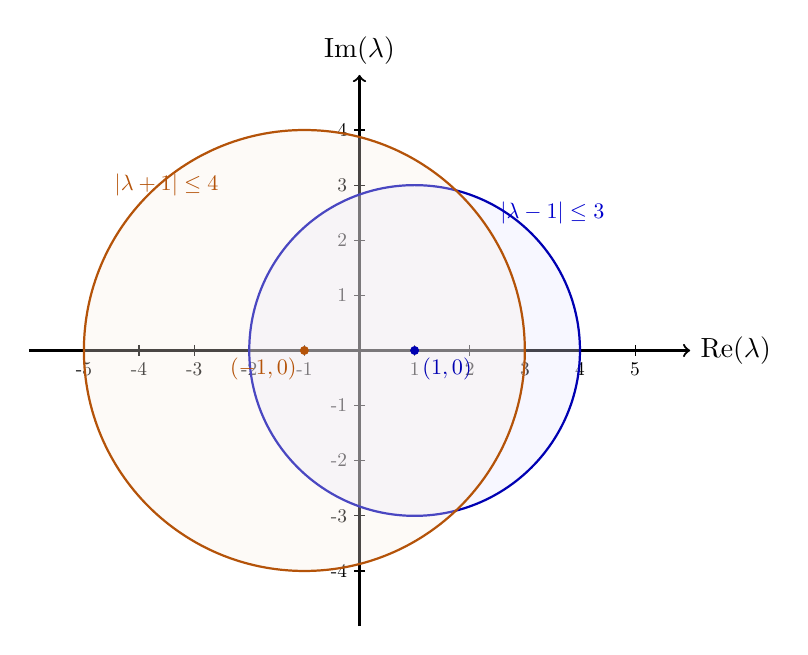
\begin{tikzpicture}[scale=0.7]
    \draw[->, thick] (-6,0) -- (6,0) node[right] {$\operatorname{Re}(\lambda)$};
    \draw[->, thick] (0,-5) -- (0,5) node[above] {$\operatorname{Im}(\lambda)$};
    \foreach \x in {-5,-4,-3,-2,-1,1,2,3,4,5}
        \draw (\x,0.1) -- (\x,-0.1) node[below,scale=0.7] {\x};
    \foreach \y in {-4,-3,-2,-1,1,2,3,4}
        \draw (0.1,\y) -- (-0.1,\y) node[left,scale=0.7] {\y};

    % Draw row discs
    \draw[thick, color=blue!70!black, fill=blue!10, fill opacity=0.3] (1,0) circle (3);
    \draw[thick, color=accent, fill=accent!10, fill opacity=0.3] (-1,0) circle (4);
    
    % Draw centers
    \filldraw[blue!70!black] (1,0) circle (2pt) node[below right,scale=0.8] {$(1,0)$};
    \filldraw[accent] (-1,0) circle (2pt) node[below left,scale=0.8] {$(-1,0)$};

    % Labels
    \node[blue!80!black,scale=0.8] at (3.5,2.5) {$|\lambda - 1| \le 3$};
    \node[accent,scale=0.8] at (-3.5,3) {$|\lambda + 1| \le 4$};
\end{tikzpicture}
\end{center}
\end{solbox}

\subsection{The Power Method for Dominant Eigenvalue}
The \textbf{Power Method} is an iterative algorithm designed to compute the numerically largest eigenvalue (dominant eigenvalue) and its corresponding eigenvector.

\begin{defbox}[Power Method Algorithm]
Given matrix $A$ and initial non-zero vector $X_0$:
\begin{enumerate}
    \item Compute $Y_{k+1} = A X_k$.
    \item Set $m_{k+1}$ as the element of $Y_{k+1}$ having maximum absolute magnitude:
    $$m_{k+1} = \operatorname{sgn}\left(\max |Y_{k+1}|\right) \cdot \max_{i} |y_{i, k+1}|$$
    \item Normalize the iterate: $X_{k+1} = \frac{1}{m_{k+1}} Y_{k+1}$.
    \item Repeat until $|m_{k+1} - m_k| < \epsilon$. Then $\lambda_{\max} \approx m_{k+1}$ and the dominant eigenvector is $X_{k+1}$.
\end{enumerate}
\end{defbox}

% --- Complete Power Method Lecture Problems (Que 1, 2, 3, 4) ---
\subsection{Complete Solutions to Power Method Problems (Pages 14--15 of Notes)}

\begin{exambox}[Classroom Worked Exercise 1: Tridiagonal Matrix (Pages 14--15 of Notes)]
Find the dominant eigenvalue and corresponding eigenvector of:
\begin{equation}
    A = \begin{bmatrix} 2 & -1 & 0 \\ -1 & 2 & -1 \\ 0 & -1 & 2 \end{bmatrix}, \qquad X_0 = \begin{bmatrix} 1 \\ 1 \\ 1 \end{bmatrix}
\end{equation}
\end{exambox}

\begin{solbox}[Complete Iterations Recorded on Pages 14--15]
\begin{center}
\small
\begin{tabular}{ccccc}
    \toprule
    $k$ & $Y_k = A X_{k-1}$ & $m_k = \max |Y_k|$ & Normalized $X_k = Y_k / m_k$ \\
    \midrule
    1 & $[1.0000, 0.0000, 1.0000]^T$ & 1.0000 & $[1.0000, 0.0000, 1.0000]^T$ \\
    2 & $[2.0000, -2.0000, 2.0000]^T$ & $-2.0000$ & $[-1.0000, 1.0000, -1.0000]^T$ \\
    3 & $[-3.0000, 4.0000, -3.0000]^T$ & 4.0000 & $[-0.7500, 1.0000, -0.7500]^T$ \\
    4 & $[-2.5000, 3.5000, -2.5000]^T$ & 3.5000 & $[-0.7143, 1.0000, -0.7143]^T$ \\
    5 & $[-2.4286, 3.4286, -2.4286]^T$ & 3.4286 & $[-0.7083, 1.0000, -0.7083]^T$ \\
    6 & $[-2.4167, 3.4167, -2.4167]^T$ & 3.4167 & $[-0.7073, 1.0000, -0.7073]^T$ \\
    7 & $[-2.4146, 3.4146, -2.4146]^T$ & 3.4146 & $[-0.7071, 1.0000, -0.7071]^T$ \\
    \bottomrule
\end{tabular}
\end{center}
\textbf{Conclusion:} Characteristic equation is $(2-\lambda)[(2-\lambda)^2 - 2] = 0$. The exact eigenvalues are $\lambda = 2, \; 2 \pm \sqrt{2}$. The method converges to the dominant eigenvalue:
$$\mathbf{\lambda_1 = 2 + \sqrt{2} \approx 3.41421, \qquad X_1 = \left[\frac{1}{\sqrt{2}}, -1, \frac{1}{\sqrt{2}}\right]^T \approx [0.7071, -1.0000, 0.7071]^T}$$

\end{solbox}

\begin{exambox}[Incomplete Lecture Exercise 2 (Page 15 of Notes)]
Find the largest eigenvalue and corresponding eigenvector of:
$$A = \begin{bmatrix} 1 & 3 & -1 \\ 3 & 2 & 4 \\ -1 & 4 & 10 \end{bmatrix}$$
\end{exambox}

\begin{solbox}[Complete Rigorous Solution]
We take initial guess $X_0 = [1, 1, 1]^T$.
\begin{center}
\small
\begin{tabular}{ccccc}
    \toprule
    $k$ & $Y_k = A X_{k-1}$ & $m_k = \max |Y_k|$ & Normalized $X_k = Y_k / m_k$ \\
    \midrule
    1 & $[3.0000, 9.0000, 13.0000]^T$ & 13.0000 & $[0.2308, 0.6923, 1.0000]^T$ \\
    2 & $[1.3077, 6.0769, 12.5385]^T$ & 12.5385 & $[0.1043, 0.4847, 1.0000]^T$ \\
    3 & $[0.5583, 5.2822, 11.8344]^T$ & 11.8344 & $[0.0472, 0.4463, 1.0000]^T$ \\
    4 & $[0.3862, 5.0343, 11.7382]^T$ & 11.7382 & $[0.0329, 0.4289, 1.0000]^T$ \\
    5 & $[0.3197, 4.9566, 11.6826]^T$ & 11.6826 & $[0.0274, 0.4243, 1.0000]^T$ \\
    6 & $[0.3002, 4.9310, 11.6697]^T$ & 11.6697 & $[0.0257, 0.4225, 1.0000]^T$ \\
    7 & $[0.2929, 4.9223, 11.6643]^T$ & 11.6643 & $[0.0251, 0.4220, 1.0000]^T$ \\
    \bottomrule
\end{tabular}
\end{center}
\textbf{Conclusion:} The dominant eigenvalue correct to 3 decimal places is $\mathbf{\lambda_1 \approx 11.662}$, with eigenvector $\mathbf{X_1 \approx [0.0251, 0.4220, 1.0000]^T}$. (Exact: $\lambda_1 \approx 11.66199$).
\end{solbox}

\begin{exambox}[Incomplete Lecture Exercise 3 (Page 15 of Notes)]
Find the largest eigenvalue and corresponding eigenvector of:
$$A = \begin{bmatrix} 1 & 6 & 1 \\ 4 & 2 & 0 \\ 0 & 0 & 3 \end{bmatrix}$$
\end{exambox}

\begin{solbox}[Complete Rigorous Solution]
Notice the upper block-triangular structure:
$$\det(A - \lambda I) = (3 - \lambda)\det\begin{bmatrix} 1-\lambda & 6 \\ 4 & 2-\lambda \end{bmatrix} = (3 - \lambda)[(1-\lambda)(2-\lambda) - 24] = (3 - \lambda)(\lambda^2 - 3\lambda - 22) = 0$$
The roots are $\lambda = 3$ and $\lambda = \frac{3 \pm \sqrt{9 + 88}}{2} = \frac{3 \pm \sqrt{97}}{2} \approx \frac{3 \pm 9.848858}{2}$.
Thus:
$$\lambda_1 = \frac{3 + \sqrt{97}}{2} \approx \mathbf{6.424429}, \qquad \lambda_2 = \frac{3 - \sqrt{97}}{2} \approx -3.424429, \qquad \lambda_3 = 3$$
The dominant eigenvalue is $\mathbf{\lambda_1 \approx 6.424429}$.
Applying the Power Method starting with $X_0 = [1, 1, 1]^T$:
\begin{center}
\small
\begin{tabular}{ccccc}
    \toprule
    $k$ & $Y_k = A X_{k-1}$ & $m_k = \max |Y_k|$ & Normalized $X_k = Y_k / m_k$ \\
    \midrule
    1 & $[8.0000, 6.0000, 3.0000]^T$ & 8.0000 & $[1.0000, 0.7500, 0.3750]^T$ \\
    2 & $[5.8750, 5.5000, 1.1250]^T$ & 5.8750 & $[1.0000, 0.9362, 0.1915]^T$ \\
    3 & $[6.8085, 5.8723, 0.5745]^T$ & 6.8085 & $[1.0000, 0.8625, 0.0844]^T$ \\
    4 & $[6.2594, 5.7250, 0.2531]^T$ & 6.2594 & $[1.0000, 0.9146, 0.0404]^T$ \\
    5 & $[6.5282, 5.8293, 0.1213]^T$ & 6.5282 & $[1.0000, 0.8929, 0.0186]^T$ \\
    6 & $[6.3762, 5.7859, 0.0558]^T$ & 6.3762 & $[1.0000, 0.9074, 0.0087]^T$ \\
    7 & $[6.4533, 5.8148, 0.0262]^T$ & 6.4533 & $[1.0000, 0.9011, 0.0041]^T$ \\
    \bottomrule
\end{tabular}
\end{center}
As $k \to \infty$, $m_k \to \mathbf{6.4244}$ and $X_k \to \mathbf{[1.0000, 0.9041, 0.0000]^T}$.
\end{solbox}

\begin{exambox}[Incomplete Lecture Exercise 4 (Page 15 of Notes)]
Find the largest eigenvalue and corresponding eigenvector of:
$$A = \begin{bmatrix} 3 & 2 & 1 \\ 2 & 3 & 2 \\ 1 & 2 & 3 \end{bmatrix}$$
\end{exambox}

\begin{solbox}[Complete Rigorous Solution]
Matrix $A$ is symmetric. The characteristic polynomial is:
$$\det(A - \lambda I) = -(\lambda - 2)(\lambda^2 - 7\lambda + 4) = 0$$
The exact eigenvalues are $\lambda = 2$ and $\lambda = \frac{7 \pm \sqrt{49 - 16}}{2} = \frac{7 \pm \sqrt{33}}{2}$.
The dominant eigenvalue is:
$$\mathbf{\lambda_1 = \frac{7 + \sqrt{33}}{2} \approx 6.372281}$$
Iterating with $X_0 = [1, 1, 1]^T$:
\begin{center}
\small
\begin{tabular}{ccccc}
    \toprule
    $k$ & $Y_k = A X_{k-1}$ & $m_k = \max |Y_k|$ & Normalized $X_k = Y_k / m_k$ \\
    \midrule
    1 & $[6.0000, 7.0000, 6.0000]^T$ & 7.0000 & $[0.8571, 1.0000, 0.8571]^T$ \\
    2 & $[5.4286, 6.4286, 5.4286]^T$ & 6.4286 & $[0.8444, 1.0000, 0.8444]^T$ \\
    3 & $[5.3778, 6.3778, 5.3778]^T$ & 6.3778 & $[0.8432, 1.0000, 0.8432]^T$ \\
    4 & $[5.3728, 6.3728, 5.3728]^T$ & 6.3728 & $[0.8431, 1.0000, 0.8431]^T$ \\
    5 & $[5.3723, 6.3723, 5.3723]^T$ & 6.3723 & $[0.8431, 1.0000, 0.8431]^T$ \\
    \bottomrule
\end{tabular}
\end{center}
\textbf{Conclusion:} Converges to $\mathbf{\lambda_1 = \frac{7 + \sqrt{33}}{2} \approx 6.37228}$ and eigenvector $\mathbf{X_1 = \left[\frac{\sqrt{33}-3}{4}, 1, \frac{\sqrt{33}-3}{4}\right]^T \approx [0.8431, 1.0000, 0.8431]^T}$.
\end{solbox}

\newpage

% =========================================================================
% MODULE 4: CALCULUS OF FINITE DIFFERENCES
% =========================================================================
\section{Calculus of Finite Differences \& Operator Algebra}

\subsection{Fundamental Operators}
Let $y = f(x)$ be tabulated at equispaced nodes $x_i = x_0 + i h$ ($i = 0, 1, \dots, n$) with step size $h > 0$. We define the following core operators:

\begin{center}
\begin{tabular}{lll}
    \toprule
    \textbf{Operator Name} & \textbf{Symbol \& Definition} & \textbf{Operator Relation} \\
    \midrule
    Forward Difference & $\Delta y(x) = y(x+h) - y(x)$ & $\Delta \equiv E - 1$ \\
    Backward Difference & $\nabla y(x) = y(x) - y(x-h)$ & $\nabla \equiv 1 - E^{-1}$ \\
    Shift Operator & $E y(x) = y(x+h)$ & $E \equiv 1 + \Delta \equiv e^{hD}$ \\
    Central Difference & $\delta y(x) = y(x + h/2) - y(x - h/2)$ & $\delta \equiv E^{1/2} - E^{-1/2}$ \\
    Averaging Operator & $\mu y(x) = \frac{1}{2}\left[y(x + h/2) + y(x - h/2)\right]$ & $\mu \equiv \frac{1}{2}(E^{1/2} + E^{-1/2})$ \\
    Differential Operator & $D y(x) = \frac{dy}{dx}$ & $hD \equiv \ln E \equiv \ln(1+\Delta)$ \\
    \bottomrule
\end{tabular}
\end{center}

\subsection{Difference Tables}
\subsubsection{Forward Difference Table}
$$\Delta^n y_r = \Delta^{n-1} y_{r+1} - \Delta^{n-1} y_r$$
\begin{center}
\begin{tabular}{cccccc}
    \toprule
    $x$ & $y$ & $\Delta y$ & $\Delta^2 y$ & $\Delta^3 y$ & $\Delta^4 y$ \\
    \midrule
    $x_0$ & $y_0$ & & & & \\
    & & $\Delta y_0$ & & & \\
    $x_1$ & $y_1$ & & $\Delta^2 y_0$ & & \\
    & & $\Delta y_1$ & & $\Delta^3 y_0$ & \\
    $x_2$ & $y_2$ & & $\Delta^2 y_1$ & & $\Delta^4 y_0$ \\
    & & $\Delta y_2$ & & $\Delta^3 y_1$ & \\
    $x_3$ & $y_3$ & & $\Delta^2 y_2$ & & \\
    & & $\Delta y_3$ & & & \\
    $x_4$ & $y_4$ & & & & \\
    \bottomrule
\end{tabular}
\end{center}

\subsubsection{Backward Difference Table}
$$\nabla^n y_r = \nabla^{n-1} y_r - \nabla^{n-1} y_{r-1}$$
\begin{center}
\begin{tabular}{cccccc}
    \toprule
    $x$ & $y$ & $\nabla y$ & $\nabla^2 y$ & $\nabla^3 y$ & $\nabla^4 y$ \\
    \midrule
    $x_0$ & $y_0$ & & & & \\
    $x_1$ & $y_1$ & $\nabla y_1$ & & & \\
    $x_2$ & $y_2$ & $\nabla y_2$ & $\nabla^2 y_2$ & & \\
    $x_3$ & $y_3$ & $\nabla y_3$ & $\nabla^2 y_3$ & $\nabla^3 y_3$ & \\
    $x_4$ & $y_4$ & $\nabla y_4$ & $\nabla^2 y_4$ & $\nabla^3 y_4$ & $\nabla^4 y_4$ \\
    \bottomrule
\end{tabular}
\end{center}

\subsection{Rigorous Proofs of Operator Identities}

\begin{theorembox}[Operator Identity 1: $\mu \delta = \sinh(hD)$]
Prove that $\mu \delta \equiv \sinh(hD)$.
\end{theorembox}
\begin{proof}
By definition, $\mu = \frac{1}{2}(E^{1/2} + E^{-1/2})$ and $\delta = E^{1/2} - E^{-1/2}$.
$$\mu \delta = \frac{1}{2}\left(E^{1/2} + E^{-1/2}\right)\left(E^{1/2} - E^{-1/2}\right) = \frac{1}{2}\left(E - E^{-1}\right)$$
Using $E = e^{hD}$ and $E^{-1} = e^{-hD}$:
$$\mu \delta = \frac{1}{2}\left(e^{hD} - e^{-hD}\right) = \sinh(hD)$$
\end{proof}

\begin{theorembox}[Operator Identity 2: $\Delta + \nabla \equiv \frac{\Delta}{\nabla} - \frac{\nabla}{\Delta}$]
Prove that $\Delta + \nabla \equiv \frac{\Delta}{\nabla} - \frac{\nabla}{\Delta}$.
\end{theorembox}
\begin{proof}
Expressing in terms of shift operator $E$: $\Delta = E - 1$ and $\nabla = 1 - E^{-1} = \frac{E - 1}{E}$.
$$\frac{\Delta}{\nabla} = \frac{E - 1}{(E-1)/E} = E, \qquad \frac{\nabla}{\Delta} = \frac{(E-1)/E}{E-1} = \frac{1}{E} = E^{-1}$$
Therefore:
$$\text{RHS} = \frac{\Delta}{\nabla} - \frac{\nabla}{\Delta} = E - E^{-1} = (E - 1) + (1 - E^{-1}) = \Delta + \nabla = \text{LHS}$$
\end{proof}

\begin{theorembox}[Operator Identity 3: $\Delta = \frac{1}{2}\delta^2 + \delta\sqrt{1 + \frac{1}{4}\delta^2}$ (Incomplete on Page 19)]
Prove that $\Delta \equiv \frac{1}{2}\delta^2 + \delta\sqrt{1 + \frac{1}{4}\delta^2}$.
\end{theorembox}
\begin{proof}
Notice that:
$$1 + \frac{1}{4}\delta^2 = 1 + \frac{1}{4}(E^{1/2} - E^{-1/2})^2 = 1 + \frac{1}{4}(E - 2 + E^{-1}) = \frac{E + 2 + E^{-1}}{4} = \left(\frac{E^{1/2} + E^{-1/2}}{2}\right)^2 = \mu^2$$
Taking the square root yields $\sqrt{1 + \frac{1}{4}\delta^2} = \mu = \frac{1}{2}(E^{1/2} + E^{-1/2})$.
Now evaluate the right-hand side:
\begin{align*}
    \text{RHS} &= \frac{1}{2}\delta^2 + \delta \mu = \frac{1}{2}(E - 2 + E^{-1}) + \frac{1}{2}(E^{1/2} - E^{-1/2})(E^{1/2} + E^{-1/2}) \\
    &= \frac{1}{2}(E - 2 + E^{-1}) + \frac{1}{2}(E - E^{-1}) \\
    &= \frac{1}{2}(2E - 2) = E - 1 = \Delta = \text{LHS}
\end{align*}
\end{proof}

\begin{theorembox}[Operator Identity 4: $\Delta^n(1/x)$ (Incomplete on Page 19)]
Evaluate $\Delta^2\left(\frac{1}{x}\right)$ and state the general formula for $\Delta^n\left(\frac{1}{x}\right)$.
\end{theorembox}
\begin{proof}
For step length $h$:
$$\Delta\left(\frac{1}{x}\right) = \frac{1}{x+h} - \frac{1}{x} = \frac{-h}{x(x+h)}$$
$$\Delta^2\left(\frac{1}{x}\right) = \Delta\left[\frac{-h}{x(x+h)}\right] = \frac{-h}{(x+h)(x+2h)} - \left[\frac{-h}{x(x+h)}\right] = -h \left[\frac{x - (x+2h)}{x(x+h)(x+2h)}\right] = \frac{2 h^2}{x(x+h)(x+2h)}$$
By induction, the general $n$-th difference is:
\begin{equation}
    \boxed{\Delta^n\left(\frac{1}{x}\right) = \frac{(-1)^n n! h^n}{x(x+h)(x+2h)\dots(x+nh)}}
\end{equation}
For unit step length $h = 1$: $\Delta^2\left(\frac{1}{x}\right) = \frac{2}{x(x+1)(x+2)}$.
\end{proof}

\begin{theorembox}[Operator Identity 5: Exponential Series Sum (Incomplete on Page 27)]
Prove that:
\begin{equation}
    e^x \left\{ y_0 + x \Delta y_0 + \frac{x^2}{2!} \Delta^2 y_0 + \dots \right\} = y_0 + x y_1 + \frac{x^2}{2!} y_2 + \dots
\end{equation}
\end{theorembox}
\begin{proof}
Express the inner series using operator notation:
$$\sum_{n=0}^\infty \frac{x^n \Delta^n}{n!} y_0 = e^{x\Delta} y_0$$
Multiplying by $e^x$:
$$\text{LHS} = e^x \cdot e^{x\Delta} y_0 = e^{x(1 + \Delta)} y_0$$
Since $1 + \Delta = E$:
$$\text{LHS} = e^{xE} y_0 = \sum_{n=0}^\infty \frac{(xE)^n}{n!} y_0 = \sum_{n=0}^\infty \frac{x^n}{n!} E^n y_0 = \sum_{n=0}^\infty \frac{x^n}{n!} y_n = y_0 + x y_1 + \frac{x^2}{2!} y_2 + \dots = \text{RHS}$$
\end{proof}

\begin{theorembox}[Operator Identity 6: Alternating Difference Identity (Incomplete on Page 28)]
Prove that:
\begin{equation}
    y_x - \Delta^2 y_x + \Delta^3 y_x - \Delta^5 y_x + \Delta^6 y_x - \Delta^8 y_x + \dots = y_x - \Delta^2 y_{x-1} + \Delta^4 y_{x-2} - \Delta^6 y_{x-3} + \dots
\end{equation}
\end{theorembox}
\begin{proof}
Consider the left-hand side operator acting on $y_x$:
$$L = 1 - \Delta^2 + \Delta^3 - \Delta^5 + \Delta^6 - \Delta^8 + \dots = (1 - \Delta^2) + \Delta^3(1 - \Delta^2) + \Delta^6(1 - \Delta^2) + \dots$$
Factoring $(1 - \Delta^2)$:
$$L = (1 - \Delta^2)(1 + \Delta^3 + \Delta^6 + \dots) = \frac{1 - \Delta^2}{1 - \Delta^3}$$
Factoring numerator and denominator:
$$L = \frac{(1 - \Delta)(1 + \Delta)}{(1 - \Delta)(1 + \Delta + \Delta^2)} = \frac{1 + \Delta}{1 + \Delta + \Delta^2} = \frac{E}{E + \Delta^2}$$
Dividing numerator and denominator by $E$:
$$L = \frac{1}{1 + \Delta^2 E^{-1}} = 1 - \Delta^2 E^{-1} + (\Delta^2 E^{-1})^2 - (\Delta^2 E^{-1})^3 + \dots = 1 - \Delta^2 E^{-1} + \Delta^4 E^{-2} - \Delta^6 E^{-3} + \dots$$
Operating on $y_x$:
$$L y_x = y_x - \Delta^2 y_{x-1} + \Delta^4 y_{x-2} - \Delta^6 y_{x-3} + \dots = \text{RHS}$$
\end{proof}

\begin{theorembox}[Operator Identity 7: Midpoint Curvature Identity (Incomplete on Page 32)]
If $\Delta^3 y_x = 0$, prove that:
\begin{equation}
    y_{x+1/2} = \frac{1}{2}(y_x + y_{x+1}) - \frac{1}{16}(\Delta^2 y_x + \Delta^2 y_{x+1})
\end{equation}
\end{theorembox}
\begin{proof}
Recall $y_{x+1/2} = E^{1/2} y_x$. Using $E = 1 + \Delta$:
$$E^{1/2} = (1 + \Delta)^{1/2} = 1 + \frac{1}{2}\Delta - \frac{1}{8}\Delta^2 + \frac{1}{16}\Delta^3 - \dots$$
Since $\Delta^3 y_x = 0$, all terms of order $\Delta^3$ and higher vanish:
$$\text{LHS} = y_{x+1/2} = \left(1 + \frac{1}{2}\Delta - \frac{1}{8}\Delta^2\right) y_x$$
Now express the RHS in terms of $\Delta$:
$$\frac{1}{2}(y_x + y_{x+1}) = \frac{1}{2}(1 + E) y_x = \frac{1}{2}(2 + \Delta) y_x = \left(1 + \frac{1}{2}\Delta\right) y_x$$
$$\frac{1}{16}(\Delta^2 y_x + \Delta^2 y_{x+1}) = \frac{1}{16}\Delta^2(1 + E) y_x = \frac{1}{16}\Delta^2(2 + \Delta) y_x = \frac{1}{8}\Delta^2 y_x + \frac{1}{16}\Delta^3 y_x = \frac{1}{8}\Delta^2 y_x$$
Subtracting:
$$\text{RHS} = \left(1 + \frac{1}{2}\Delta\right) y_x - \frac{1}{8}\Delta^2 y_x = \left(1 + \frac{1}{2}\Delta - \frac{1}{8}\Delta^2\right) y_x = \text{LHS}$$
\end{proof}

\begin{theorembox}[Operator Identity 8: Binomial Shift Identity (Page 26 of Notes)]
Prove that:
\begin{multline}
    y_x - \frac{1}{8}\Delta^2 y_{x-1} + \frac{1 \cdot 3}{8 \cdot 16}\Delta^4 y_{x-2} - \frac{1 \cdot 3 \cdot 5}{8 \cdot 16 \cdot 24}\Delta^6 y_{x-3} + \dots \\
    = y_{x+1/2} - \frac{1}{2}\Delta y_{x+1/2} + \frac{1}{4}\Delta^2 y_{x+1/2} - \frac{1}{8}\Delta^3 y_{x+1/2} + \dots
\end{multline}
\end{theorembox}
\begin{proof}
Express the left-hand side using the backward shift operator $E^{-1}$:
\begin{align*}
    \text{LHS} &= \left[ 1 - \frac{1}{8}\Delta^2 E^{-1} + \frac{1 \cdot 3}{8 \cdot 16}\Delta^4 E^{-2} - \frac{1 \cdot 3 \cdot 5}{8 \cdot 16 \cdot 24}\Delta^6 E^{-3} + \dots \right] y_x \\
    &= \left[ 1 - \frac{1}{2}\left(\frac{\Delta^2 E^{-1}}{4}\right) + \frac{\frac{1}{2}\cdot\frac{3}{2}}{2!}\left(\frac{\Delta^2 E^{-1}}{4}\right)^2 - \frac{\frac{1}{2}\cdot\frac{3}{2}\cdot\frac{5}{2}}{3!}\left(\frac{\Delta^2 E^{-1}}{4}\right)^3 + \dots \right] y_x
\end{align*}
This is precisely the binomial expansion of $(1 + u)^{-1/2}$ for $u = \frac{\Delta^2 E^{-1}}{4}$:
\begin{align*}
    \text{LHS} &= \left( 1 + \frac{\Delta^2}{4E} \right)^{-1/2} y_x = \left( \frac{4E + \Delta^2}{4E} \right)^{-1/2} y_x \\
    &= \frac{(4E + \Delta^2)^{-1/2}}{(4E)^{-1/2}} y_x = 2 E^{1/2} (4E + \Delta^2)^{-1/2} y_x = 2(4E + \Delta^2)^{-1/2} y_{x+1/2}
\end{align*}
Using the operator equivalence $E \equiv 1 + \Delta$:
$$4E + \Delta^2 = 4(1 + \Delta) + \Delta^2 = \Delta^2 + 4\Delta + 4 = (\Delta + 2)^2$$
Substituting into the expression:
$$\text{LHS} = 2\left[ (\Delta + 2)^2 \right]^{-1/2} y_{x+1/2} = 2(\Delta + 2)^{-1} y_{x+1/2} = \frac{2}{2\left(1 + \frac{\Delta}{2}\right)} y_{x+1/2} = \left(1 + \frac{\Delta}{2}\right)^{-1} y_{x+1/2}$$
Expanding $(1 + \Delta/2)^{-1}$ as a geometric series:
\begin{align*}
    \text{LHS} &= \left[ 1 - \frac{\Delta}{2} + \left(\frac{\Delta}{2}\right)^2 - \left(\frac{\Delta}{2}\right)^3 + \dots \right] y_{x+1/2} \\
    &= y_{x+1/2} - \frac{1}{2}\Delta y_{x+1/2} + \frac{1}{4}\Delta^2 y_{x+1/2} - \frac{1}{8}\Delta^3 y_{x+1/2} + \dots = \text{RHS}
\end{align*}
\end{proof}

\begin{theorembox}[Operator Identity 9: Alternating Difference Series Summation (Page 29 of Notes)]
Evaluate the sum of the operator series:
\begin{equation}
    S = 1 \cdot 2 \Delta x^n - 2 \cdot 3 \Delta^2 x^n + 3 \cdot 4 \Delta^3 x^n - 4 \cdot 5 \Delta^4 x^n + \dots
\end{equation}
\end{theorembox}
\begin{proof}
Operating by $\Delta$ on $S$:
\begin{align*}
    S &= 1 \cdot 2 \Delta x^n - 2 \cdot 3 \Delta^2 x^n + 3 \cdot 4 \Delta^3 x^n - 4 \cdot 5 \Delta^4 x^n + \dots \\
    \Delta S &= \phantom{1 \cdot 2 \Delta x^n} + 1 \cdot 2 \Delta^2 x^n - 2 \cdot 3 \Delta^3 x^n + 3 \cdot 4 \Delta^4 x^n - \dots
\end{align*}
Adding the two equations:
\begin{align*}
    (1 + \Delta)S &= 1 \cdot 2 \Delta x^n - (6 - 2)\Delta^2 x^n + (12 - 6)\Delta^3 x^n - (20 - 12)\Delta^4 x^n + \dots \\
    &= 2\Delta x^n - 4\Delta^2 x^n + 6\Delta^3 x^n - 8\Delta^4 x^n + \dots \\
    &= 2\Delta \left[ 1 - 2\Delta + 3\Delta^2 - 4\Delta^3 + \dots \right] x^n
\end{align*}
Recall that $(1 + \Delta)^{-2} = 1 - 2\Delta + 3\Delta^2 - 4\Delta^3 + \dots$. Therefore:
$$(1 + \Delta)S = 2\Delta (1 + \Delta)^{-2} x^n \implies S = 2\Delta (1 + \Delta)^{-3} x^n$$
Using $E = 1 + \Delta$ and $\Delta = E - 1$:
$$S = 2(E - 1)E^{-3} x^n = 2(E^{-2} - E^{-3}) x^n = 2\left[ E^{-2} x^n - E^{-3} x^n \right]$$
For step size $h$, $E^{-k} f(x) = f(x - kh)$:
\begin{equation}
    \boxed{S = 2\left[ (x - 2h)^n - (x - 3h)^n \right]}
\end{equation}
For unit step length $h = 1$: $S = 2\left[(x - 2)^n - (x - 3)^n\right]$.
\end{proof}

\subsection{Fundamental Theorem of Finite Differences}
\begin{theorembox}[Fundamental Theorem of Finite Differences]
The $n$-th forward difference of a polynomial $P_n(x)$ of degree $n$ with step size $h$ is constant and equal to $a_0 n! h^n$, and all higher differences are identically zero:
\begin{equation}
    \Delta^n P_n(x) = a_0 n! h^n = \text{constant}, \qquad \Delta^{n+k} P_n(x) = 0 \quad (k \ge 1)
\end{equation}
\end{theorembox}

\subsection{Missing Value Problems}

\begin{exambox}[Classroom Problem: Single Missing Value with Error Analysis (Page 22 of Notes)]
Find the missing entry $y_3$ in the following data table:
\begin{center}
\begin{tabular}{cccccc}
    \toprule
    $x$ & 0 & 1 & 2 & 3 & 4 \\
    $y$ & 1 & 3 & 9 & $y_3$ & 81 \\
    \bottomrule
\end{tabular}
\end{center}
Explain why the interpolated value differs from $3^3 = 27$.
\end{exambox}

\begin{solbox}[Step-by-Step Solution]
Since four values are given ($y_0 = 1, y_1 = 3, y_2 = 9, y_4 = 81$), the underlying function can be modeled by a polynomial of degree 3. By the Fundamental Theorem of Finite Differences, the fourth differences vanish:
$$\Delta^4 y_0 = 0 \iff (E - 1)^4 y_0 = 0$$
Expanding the binomial operator $(E - 1)^4 = E^4 - 4E^3 + 6E^2 - 4E + 1$:
$$y_4 - 4y_3 + 6y_2 - 4y_1 + y_0 = 0$$
Isolating the missing entry $y_3$:
$$y_3 = \frac{1}{4}\left(y_4 + 6y_2 - 4y_1 + y_0\right)$$
Substitute the tabulated values:
$$y_3 = \frac{1}{4}\left[81 + 6(9) - 4(3) + 1\right] = \frac{1}{4}\left[81 + 54 - 12 + 1\right] = \frac{124}{4} = \mathbf{31}$$

\textbf{Mathematical Note on Discrepancy (Recorded in Lecture Notes):}
Notice that the tabulated values $y = [1, 3, 9, \dots, 81]$ represent the exponential function $f(x) = 3^x$, for which $f(3) = 3^3 = 27$. However, the finite difference method assumes $f(x)$ is a cubic polynomial. Because $3^x$ is \emph{not} a polynomial, the cubic polynomial passing through $(0,1), (1,3), (2,9), (4,81)$ produces $y_3 = 31$, incurring a truncation discrepancy of $31 - 27 = 4$.
\end{solbox}

\begin{exambox}[Incomplete Lecture Problem: Two Missing Values (Pages 22--23 of Notes)]
Find the missing entries $y_1$ and $y_3$ in the following data table:
\begin{center}
\begin{tabular}{ccccccc}
    \toprule
    $x$ & 0 & 1 & 2 & 3 & 4 & 5 \\
    $y$ & 1 & $y_1$ & 8 & $y_3$ & 19 & 31 \\
    \bottomrule
\end{tabular}
\end{center}
\end{exambox}

\begin{solbox}[Complete Rigorous Solution]
Since four functional values are given ($y_0 = 1, y_2 = 8, y_4 = 19, y_5 = 31$), the underlying function can be represented by a polynomial of degree 3.
By the Fundamental Theorem of Finite Differences, the fourth differences are zero:
\begin{align}
    \Delta^4 y_0 &= 0 \iff (E - 1)^4 y_0 = 0 \label{eq:miss1} \\
    \Delta^4 y_1 &= 0 \iff (E - 1)^4 y_1 = 0 \label{eq:miss2}
\end{align}
Expanding the binomial operator $(E - 1)^4 = E^4 - 4E^3 + 6E^2 - 4E + 1$:
\begin{align}
    y_4 - 4y_3 + 6y_2 - 4y_1 + y_0 &= 0 \label{eq:m1} \\
    y_5 - 4y_4 + 6y_3 - 4y_2 + y_1 &= 0 \label{eq:m2}
\end{align}
Substitute the known values into \eqref{eq:m1}:
$$19 - 4y_3 + 6(8) - 4y_1 + 1 = 0 \implies 68 - 4y_1 - 4y_3 = 0 \implies \mathbf{y_1 + y_3 = 17}$$
Substitute into \eqref{eq:m2}:
$$31 - 4(19) + 6y_3 - 4(8) + y_1 = 0 \implies 31 - 76 + 6y_3 - 32 + y_1 = 0 \implies \mathbf{y_1 + 6y_3 = 77}$$
Subtracting the two equations:
$$(y_1 + 6y_3) - (y_1 + y_3) = 77 - 17 \implies 5y_3 = 60 \implies \mathbf{y_3 = 12}$$
Substituting back:
$$y_1 = 17 - 12 \implies \mathbf{y_1 = 5}$$

\textbf{Verification via Difference Table:}
The complete dataset is $y = [1, 5, 8, 12, 19, 31]$.
\begin{itemize}
    \item First differences $\Delta y$: $4, 3, 4, 7, 12$.
    \item Second differences $\Delta^2 y$: $-1, 1, 3, 5$.
    \item Third differences $\Delta^3 y$: $2, 2, 2$ (constant!).
    \item Fourth differences $\Delta^4 y$: $0, 0$ (verified!).
\end{itemize}
\textbf{Final Answer:} $\mathbf{y_1 = 5, \quad y_3 = 12}$.
\end{solbox}

\subsection{Factorial Notation \& Polynomial Conversion}
\begin{defbox}[Factorial Polynomial]
The factorial polynomial of degree $n$ with step length $h=1$ is defined as:
\begin{equation}
    [x]^n = x(x - 1)(x - 2)\dots(x - n + 1), \qquad [x]^0 = 1
\end{equation}
Its forward difference mirrors standard differential calculus:
\begin{equation}
    \Delta [x]^n = n [x]^{n-1}, \qquad \Delta^{-1} [x]^n = \frac{[x]^{n+1}}{n+1} + C
\end{equation}
\end{defbox}

\begin{exambox}[Classroom Problem 1: Interval of Differencing (Page 24 of Notes)]
Find the interval of differencing $h$ if $\Delta x^2 = x + \frac{1}{4}$.
\end{exambox}

\begin{solbox}[Step-by-Step Solution]
By definition of the forward difference operator with step length $h$:
$$\Delta x^2 = (x + h)^2 - x^2 = x^2 + 2hx + h^2 - x^2 = 2hx + h^2$$
We are given that $\Delta x^2 = x + \frac{1}{4}$. Equating coefficients of like powers of $x$:
\begin{align*}
    x^1&: \quad 2h = 1 \implies h = \frac{1}{2} \\
    x^0&: \quad h^2 = \frac{1}{4} \implies h = \pm \frac{1}{2}
\end{align*}
Both conditions are consistently satisfied by:
$$\mathbf{h = \frac{1}{2}}$$
Hence, the required interval of differencing is $\mathbf{h = 1/2}$.
\end{solbox}

\begin{exambox}[Classroom Problem 2: Factorial Form of Cubic Polynomial (Page 24 of Notes)]
Express $y = 2x^3 - 3x^2 + 3x - 1$ in factorial notation and determine its successive differences $\Delta y, \Delta^2 y, \Delta^3 y, \Delta^4 y$.
\end{exambox}

\begin{solbox}[Solution via Synthetic Division]
Let $y = A[x]^3 + B[x]^2 + C[x] + D$.
At $x = 0$, $D = -1$.
We find coefficients $C, B, A$ by dividing successively by $x = 1, 2$:
\begin{center}
\begin{tabular}{c|cccc}
    & 2 & $-3$ & 3 & $-1$ \\
    1 & & 2 & $-1$ & 2 \\
    \hline
    & 2 & $-1$ & $\mathbf{2 = C}$ & $\mathbf{-1 = D}$ \\
    2 & & 4 & & \\
    \hline
    & $\mathbf{2 = A}$ & $\mathbf{3 = B}$ & &
\end{tabular}
\end{center}
Hence, the factorial representation is:
\begin{equation}
    \boxed{y = 2[x]^3 + 3[x]^2 + 2[x] - 1}
\end{equation}
\textbf{Successive Differences (for $h = 1$):}
\begin{align*}
    \Delta y &= 2 \cdot 3[x]^2 + 3 \cdot 2[x] + 2 = 6[x]^2 + 6[x] + 2 \\
    \Delta^2 y &= 6 \cdot 2[x] + 6 = 12[x] + 6 \\
    \Delta^3 y &= 12 \cdot 1 = 12 \\
    \Delta^4 y &= 0
\end{align*}
\end{solbox}

% --- Incomplete Exercise on Page 25 Completed ---
\begin{exambox}[Incomplete Lecture Exercise (Page 25 of Notes)]
Express $f(x) = 11x^4 + 5x^3 + x - 15$ in factorial notation and compute all successive differences.
\end{exambox}

\begin{solbox}[Complete Rigorous Solution]
Notice the polynomial includes a missing second-degree term:
$$f(x) = 11x^4 + 5x^3 + 0x^2 + 1x - 15$$
Let $f(x) = A[x]^4 + B[x]^3 + C[x]^2 + D[x] + E$.
Setting $x = 0$ immediately gives $\mathbf{E = -15}$.
We determine coefficients $D, C, B, A$ using sequential Horner synthetic division:
\begin{center}
\begin{tabular}{c|ccccc}
    & 11 & 5 & 0 & 1 \\
    1 & & 11 & 16 & 16 \\
    \hline
    & 11 & 16 & 16 & $\mathbf{17 = D}$ \\
    2 & & 22 & 76 & \\
    \hline
    & 11 & 38 & $\mathbf{92 = C}$ & \\
    3 & & 33 & & \\
    \hline
    & $\mathbf{11 = A}$ & $\mathbf{71 = B}$ & &
\end{tabular}
\end{center}
Thus, the factorial representation is:
\begin{equation}
    \boxed{f(x) = 11[x]^4 + 71[x]^3 + 92[x]^2 + 17[x] - 15}
\end{equation}
\textbf{Successive Differences:}
\begin{align*}
    \Delta f(x) &= 44[x]^3 + 213[x]^2 + 184[x] + 17 \\
    \Delta^2 f(x) &= 132[x]^2 + 426[x] + 184 \\
    \Delta^3 f(x) &= 264[x] + 426 \\
    \Delta^4 f(x) &= 264 \\
    \Delta^5 f(x) &= 0
\end{align*}
\end{solbox}

\subsection{Summation of Series using Finite Differences}

\begin{exambox}[Incomplete Lecture Problem (Page 29 of Notes)]
Find the sum of $n$ terms of the series:
$$S_n = 2\cdot 5 + 5\cdot 8 + 8\cdot 11 + 11\cdot 14 + \dots$$
\end{exambox}

\begin{solbox}[Complete Rigorous Solution]
The general $r$-th term is:
$$T_r = (3r - 1)(3r + 2) = 9r^2 + 3r - 2$$
Converting $r^2$ into factorial notation ($r^2 = [r]^2 + [r]$):
$$T_r = 9([r]^2 + [r]) + 3[r] - 2 = 9[r]^2 + 12[r] - 2$$
Using the antidifference summation formula $\sum_{r=1}^n T_r = \left[ \Delta^{-1} T_r \right]_1^{n+1}$:
\begin{align*}
    S_n &= \left[ 9 \frac{[r]^3}{3} + 12 \frac{[r]^2}{2} - 2[r] \right]_1^{n+1} = \left[ 3[r]^3 + 6[r]^2 - 2[r] \right]_1^{n+1} \\
    &= \left\{ 3(n+1)n(n-1) + 6(n+1)n - 2(n+1) \right\} - \left\{ 0 + 0 - 2(1) \right\} \\
    &= (n+1)\left[ 3n^2 - 3n + 6n - 2 \right] + 2 = (n+1)(3n^2 + 3n - 2) + 2 \\
    &= 3n^3 + 6n^2 + n
\end{align*}
\begin{equation}
    \boxed{S_n = n(3n^2 + 6n + 1)}
\end{equation}
\textbf{Verification:}
For $n=1$: $S_1 = 1(3 + 6 + 1) = 10 = 2\cdot 5$.
For $n=2$: $S_2 = 2(12 + 12 + 1) = 50 = 10 + 40$.
For $n=3$: $S_3 = 3(27 + 18 + 1) = 138 = 50 + 88$. Matches perfectly!
\end{solbox}

\begin{exambox}[Incomplete Lecture Problem (Page 30 of Notes)]
Find the $n$-th term of the sequence: $1, 4, 10, 20, 35, 56, \dots$
\end{exambox}

\begin{solbox}[Complete Rigorous Solution]
Construct the difference table for the sequence $u_1, u_2, u_3, \dots$:
\begin{itemize}
    \item $u$: $1, 4, 10, 20, 35, 56$
    \item $\Delta u$: $3, 6, 10, 15, 21$
    \item $\Delta^2 u$: $3, 4, 5, 6$
    \item $\Delta^3 u$: $1, 1, 1$ (constant $\Delta^3 u_1 = 1$)
    \item $\Delta^4 u$: $0$.
\end{itemize}
Using $T_n = E^{n-1} u_1 = (1 + \Delta)^{n-1} u_1$:
\begin{align*}
    T_n &= u_1 + (n-1)\Delta u_1 + \frac{(n-1)(n-2)}{2!}\Delta^2 u_1 + \frac{(n-1)(n-2)(n-3)}{3!}\Delta^3 u_1 \\
    &= 1 + 3(n-1) + \frac{3}{2}(n-1)(n-2) + \frac{1}{6}(n-1)(n-2)(n-3)
\end{align*}
Combining terms over common denominator 6:
\begin{align*}
    T_n &= \frac{1}{6}\left[ 6 + 18(n-1) + 9(n^2 - 3n + 2) + (n^3 - 6n^2 + 11n - 6) \right] \\
    &= \frac{1}{6}\left[ n^3 + 3n^2 + 2n \right] = \frac{n(n+1)(n+2)}{6} = \binom{n+2}{3}
\end{align*}
\begin{equation}
    \boxed{T_n = \frac{n(n+1)(n+2)}{6} = \binom{n+2}{3}}
\end{equation}
\end{solbox}

\begin{exambox}[Incomplete Lecture Problem: Sum of Squares of First $n$ Natural Numbers (Page 30 of Notes)]
Evaluate the sum of the series using finite difference methods:
\begin{equation}
    S_n = 1^2 + 2^2 + 3^2 + \dots + n^2
\end{equation}
\end{exambox}

\begin{solbox}[Solution via Factorial Polynomials]
Convert $r^2$ into factorial polynomials:
$$r^2 = [r]^2 + [r]$$
Applying the summation formula $\sum_{r=1}^n T_r = \left[ \Delta^{-1} T_r \right]_1^{n+1}$:
\begin{align*}
    S_n &= \sum_{r=1}^n \left( [r]^2 + [r] \right) = \left[ \frac{[r]^3}{3} + \frac{[r]^2}{2} \right]_1^{n+1} \\
    &= \left\{ \frac{(n+1)n(n-1)}{3} + \frac{(n+1)n}{2} \right\} - \{ 0 + 0 \} \\
    &= \frac{n(n+1)}{6} \left[ 2(n-1) + 3 \right] = \frac{n(n+1)(2n+1)}{6}
\end{align*}
\begin{equation}
    \boxed{\sum_{r=1}^n r^2 = \frac{n(n+1)(2n+1)}{6}}
\end{equation}
\end{solbox}

\begin{exambox}[Classroom Problem: Sum of Cubes via Operator Formula (Page 31 of Notes)]
Evaluate the sum of the first $n$ cubes:
\begin{equation}
    S_n = 1^3 + 2^3 + 3^3 + \dots + n^3
\end{equation}
using the finite difference summation operator $\frac{(1 + \Delta)^n - 1}{\Delta} y_0$.
\end{exambox}

\begin{solbox}[Complete Operator Derivation Recorded on Page 31]
Let $y_r = (r + 1)^3$ for $r = 0, 1, \dots, n-1$, so that $S_n = y_0 + y_1 + \dots + y_{n-1}$.
Expressing in terms of shift operator $E$:
$$S_n = (1 + E + E^2 + \dots + E^{n-1})y_0 = \frac{E^n - 1}{E - 1}y_0$$
Since $E = 1 + \Delta$ and $E - 1 = \Delta$:
$$S_n = \frac{(1 + \Delta)^n - 1}{\Delta} y_0$$
Expanding $(1 + \Delta)^n$ using the binomial theorem:
\begin{align*}
    S_n &= \frac{1}{\Delta}\left[ 1 + n\Delta + \frac{n(n-1)}{2!}\Delta^2 + \frac{n(n-1)(n-2)}{3!}\Delta^3 + \frac{n(n-1)(n-2)(n-3)}{4!}\Delta^4 + \dots - 1 \right] y_0 \\
    &= n y_0 + \frac{n(n-1)}{2!}\Delta y_0 + \frac{n(n-1)(n-2)}{3!}\Delta^2 y_0 + \frac{n(n-1)(n-2)(n-3)}{4!}\Delta^3 y_0 + \dots
\end{align*}
Difference table for $y_x = (x+1)^3$:
\begin{center}
\begin{tabular}{c|ccccc}
    \toprule
    $x$ & $y = (x+1)^3$ & $\Delta y$ & $\Delta^2 y$ & $\Delta^3 y$ & $\Delta^4 y$ \\
    \midrule
    0 & $\mathbf{1 = y_0}$ & & & & \\
    & & $\mathbf{7 = \Delta y_0}$ & & & \\
    1 & 8 & & $\mathbf{12 = \Delta^2 y_0}$ & & \\
    & & 19 & & $\mathbf{6 = \Delta^3 y_0}$ & \\
    2 & 27 & & 18 & & $\mathbf{0 = \Delta^4 y_0}$ \\
    & & 37 & & 6 & \\
    3 & 64 & & 24 & & 0 \\
    \bottomrule
\end{tabular}
\end{center}
Substituting $y_0 = 1$, $\Delta y_0 = 7$, $\Delta^2 y_0 = 12$, $\Delta^3 y_0 = 6$, and $\Delta^k y_0 = 0$ ($k \ge 4$):
\begin{align*}
    S_n &= n(1) + \frac{n(n-1)}{2}(7) + \frac{n(n-1)(n-2)}{6}(12) + \frac{n(n-1)(n-2)(n-3)}{24}(6) \\
    &= n + \frac{7}{2}n(n-1) + 2n(n-1)(n-2) + \frac{1}{4}n(n-1)(n-2)(n-3) \\
    &= \frac{n}{4}\left[ 4 + 14(n-1) + 8(n-1)(n-2) + (n-1)(n-2)(n-3) \right] \\
    &= \frac{n}{4}\left[ 4 + 14n - 14 + 8(n^2 - 3n + 2) + (n^3 - 6n^2 + 11n - 6) \right] \\
    &= \frac{n}{4}\left[ n^3 + 2n^2 + n \right] = \frac{n^2(n+1)^2}{4} = \left[\frac{n(n+1)}{2}\right]^2
\end{align*}
\begin{equation}
    \boxed{\sum_{r=1}^n r^3 = \left[\frac{n(n+1)}{2}\right]^2}
\end{equation}
\end{solbox}

\newpage

% =========================================================================
% MODULE 5: INTERPOLATION WITH EQUIDISTANT NODES
% =========================================================================
\section{Interpolation with Equidistant Nodes}

\subsection{Newton's Forward Interpolation Formula}
Let $y = f(x)$ be known at $n+1$ equidistant points $x_0, x_1, \dots, x_n$ with spacing $h$. Let $x = x_0 + p h$ be an interpolation point near the beginning of the table, where $p = \frac{x - x_0}{h} \in \mathbb{R}$.

Using the shift operator $E = 1 + \Delta$:
\begin{equation}
    y(x) = E^p y_0 = (1 + \Delta)^p y_0
\end{equation}
Expanding $(1 + \Delta)^p$ via the binomial theorem:
\begin{equation}
    \boxed{y(x) = y_0 + p \Delta y_0 + \frac{p(p-1)}{2!} \Delta^2 y_0 + \frac{p(p-1)(p-2)}{3!} \Delta^3 y_0 + \dots + \frac{p(p-1)\dots(p-n+1)}{n!} \Delta^n y_0}
\end{equation}
The truncation error is given by:
\begin{equation}
    R_n(x) = \frac{p(p-1)\dots(p-n)}{(n+1)!} h^{n+1} f^{(n+1)}(\xi), \qquad \xi \in (x_0, x_n)
\end{equation}

\subsection{Newton's Backward Interpolation Formula (Completed from Page 32)}
When the point $x$ lies near the end of the table ($x_n$), we set:
\begin{equation}
    x = x_n + p h \iff p = \frac{x - x_n}{h}
\end{equation}
Using the backward difference operator $\nabla = 1 - E^{-1} \iff E^{-1} = 1 - \nabla \iff E = (1 - \nabla)^{-1}$:
\begin{equation}
    y(x) = E^p y_n = (1 - \nabla)^{-p} y_n
\end{equation}
Expanding $(1 - \nabla)^{-p}$ via negative binomial series:
\begin{equation}
    (1 - \nabla)^{-p} = 1 + (-p)(-\nabla) + \frac{(-p)(-p-1)}{2!}(-\nabla)^2 + \dots = 1 + p\nabla + \frac{p(p+1)}{2!}\nabla^2 + \dots
\end{equation}
Hence, we obtain the \textbf{Newton's Backward Interpolation Formula}:
\begin{equation}
    \boxed{y(x) = y_n + p \nabla y_n + \frac{p(p+1)}{2!} \nabla^2 y_n + \frac{p(p+1)(p+2)}{3!} \nabla^3 y_n + \dots + \frac{p(p+1)\dots(p+n-1)}{n!} \nabla^n y_n}
\end{equation}
The truncation error is:
\begin{equation}
    R_n(x) = \frac{p(p+1)\dots(p+n)}{(n+1)!} h^{n+1} f^{(n+1)}(\xi'), \qquad \xi' \in (x_0, x_n)
\end{equation}

\subsection{Selection Criteria: Forward vs. Backward Interpolation}
\begin{center}
\begin{tabular}{p{3.5cm}p{6cm}p{6cm}}
    \toprule
    \textbf{Criterion} & \textbf{Newton's Forward Formula} & \textbf{Newton's Backward Formula} \\
    \midrule
    \textbf{Target Point Position} & Near the start of the table ($x \approx x_0$) & Near the end of the table ($x \approx x_n$) \\
    \textbf{Parameter $p$} & $p = \frac{x - x_0}{h}$, ideally $0 \le p < 1$ & $p = \frac{x - x_n}{h}$, ideally $-1 < p \le 0$ \\
    \textbf{Operators Used} & Forward differences $\Delta, \Delta^2, \dots$ & Backward differences $\nabla, \nabla^2, \dots$ \\
    \textbf{Reference Row} & Top row of difference table ($y_0$) & Bottom row of difference table ($y_n$) \\
    \textbf{Extrapolation} & Extrapolating to the left ($x < x_0$) & Extrapolating to the right ($x > x_n$) \\
    \bottomrule
\end{tabular}
\end{center}

\vspace{10pt}
\hrule
\begin{center}
    {\small\color{subtle} $\blacksquare$ End of Lecture Notes $\bullet$ Typeset in \LaTeX{} for Academic Excellence $\bullet$ BHU Semester 5}
\end{center}

\end{document}
